\section{Model B}

\subsection{Multilevel Model}

\begin{frame}{Multilevel Model}
    We fit an \textbf{intercept only} model as:

    \begin{equation*}
        \mathrm{SAP}
            = \beta_{\mathrm{Year}}
            + \gamma_{\, \mathrm{Year}, \, \mathrm{Region}}
            + \epsilon
    \end{equation*}

    where
    
    \begin{itemize}
        \item $\beta$ represents a population effect, by year;
        \item $\gamma$ represents a region-specific effect, by year;
        \item $\epsilon$ is a noise term.
    \end{itemize}
\end{frame}

\begin{frame}{Population Effect}
    \begin{figure}[H]
        \centering
        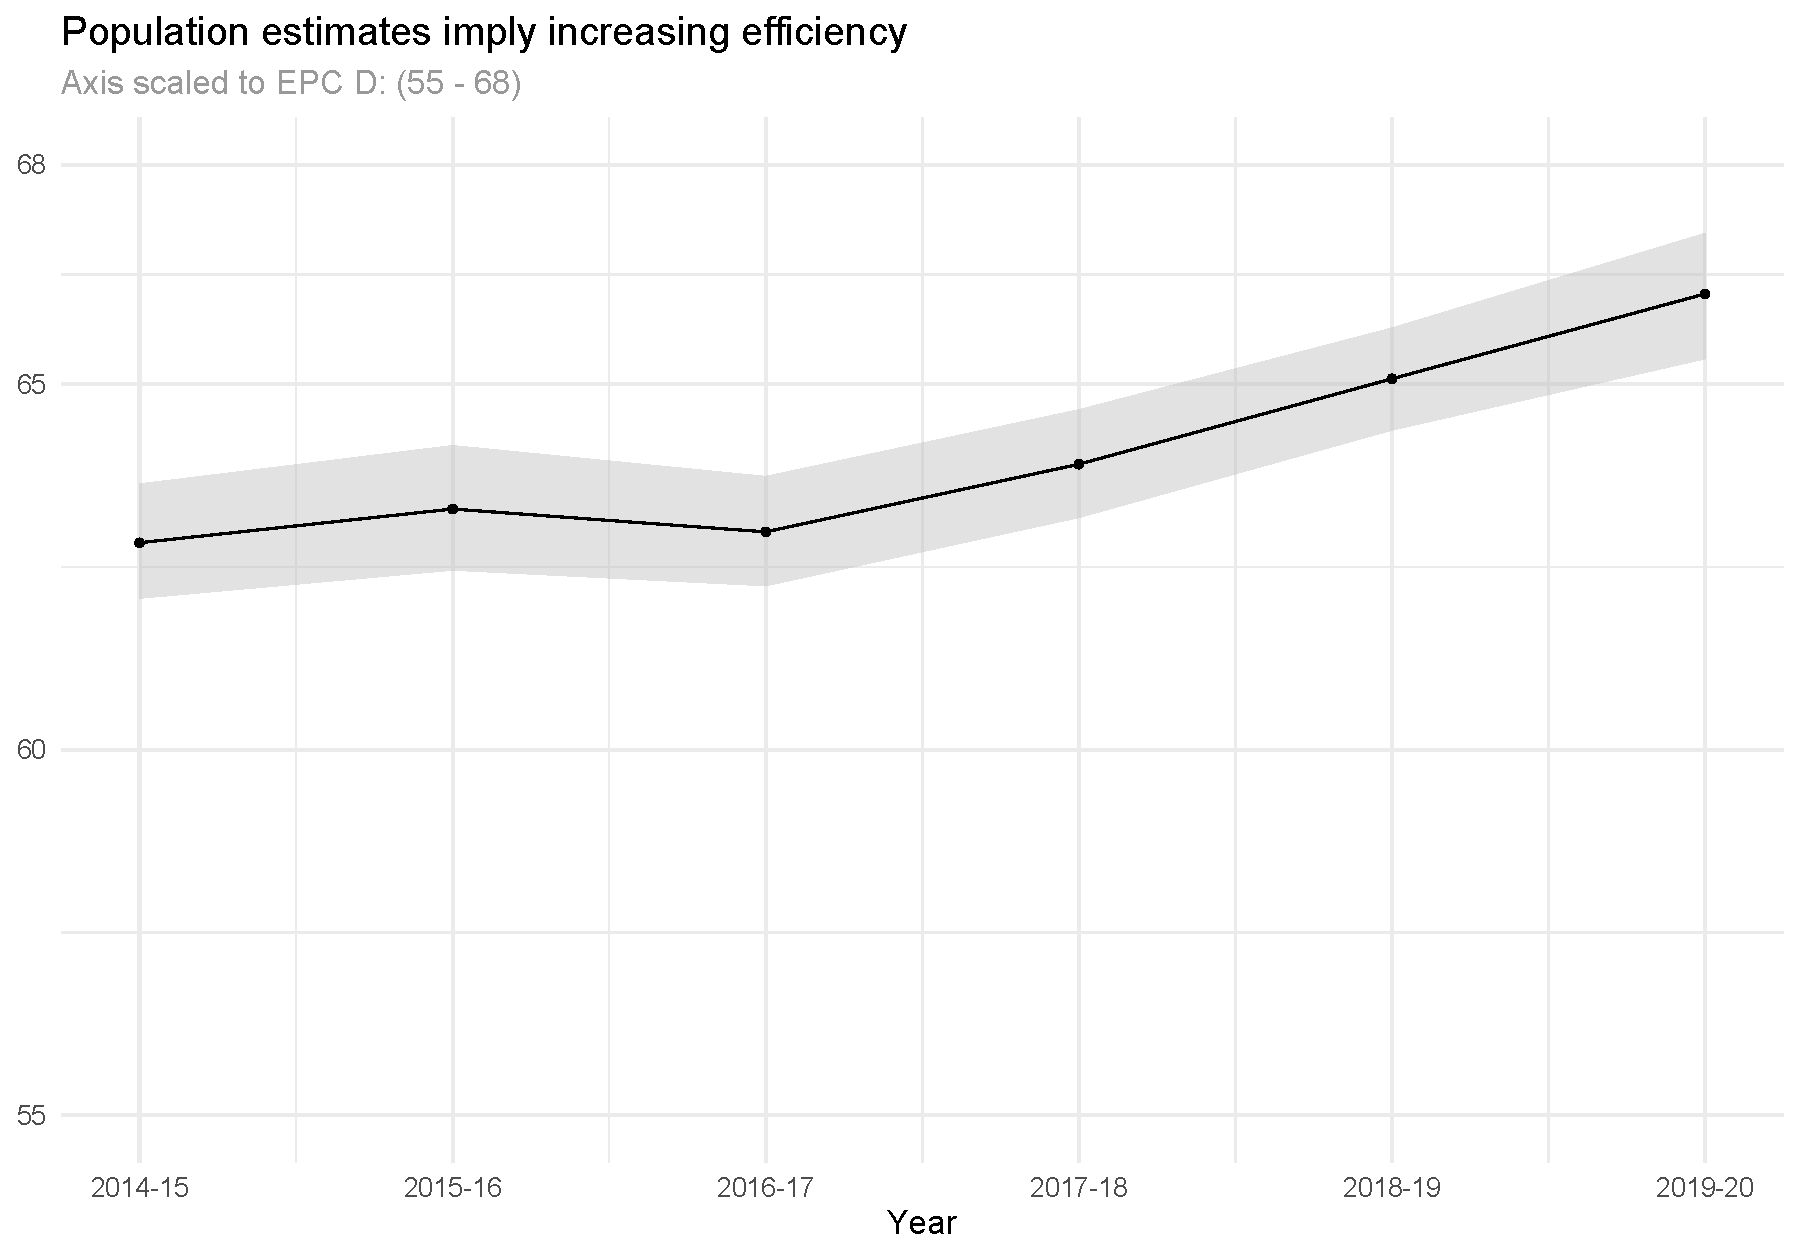
\includegraphics
            [width = \textwidth]
            {fig3_1-1}
        \label{fig:fig3_1-1}
    \end{figure}
\end{frame}

\begin{frame}{Regional Effects}
    \begin{figure}[H]
        \centering
        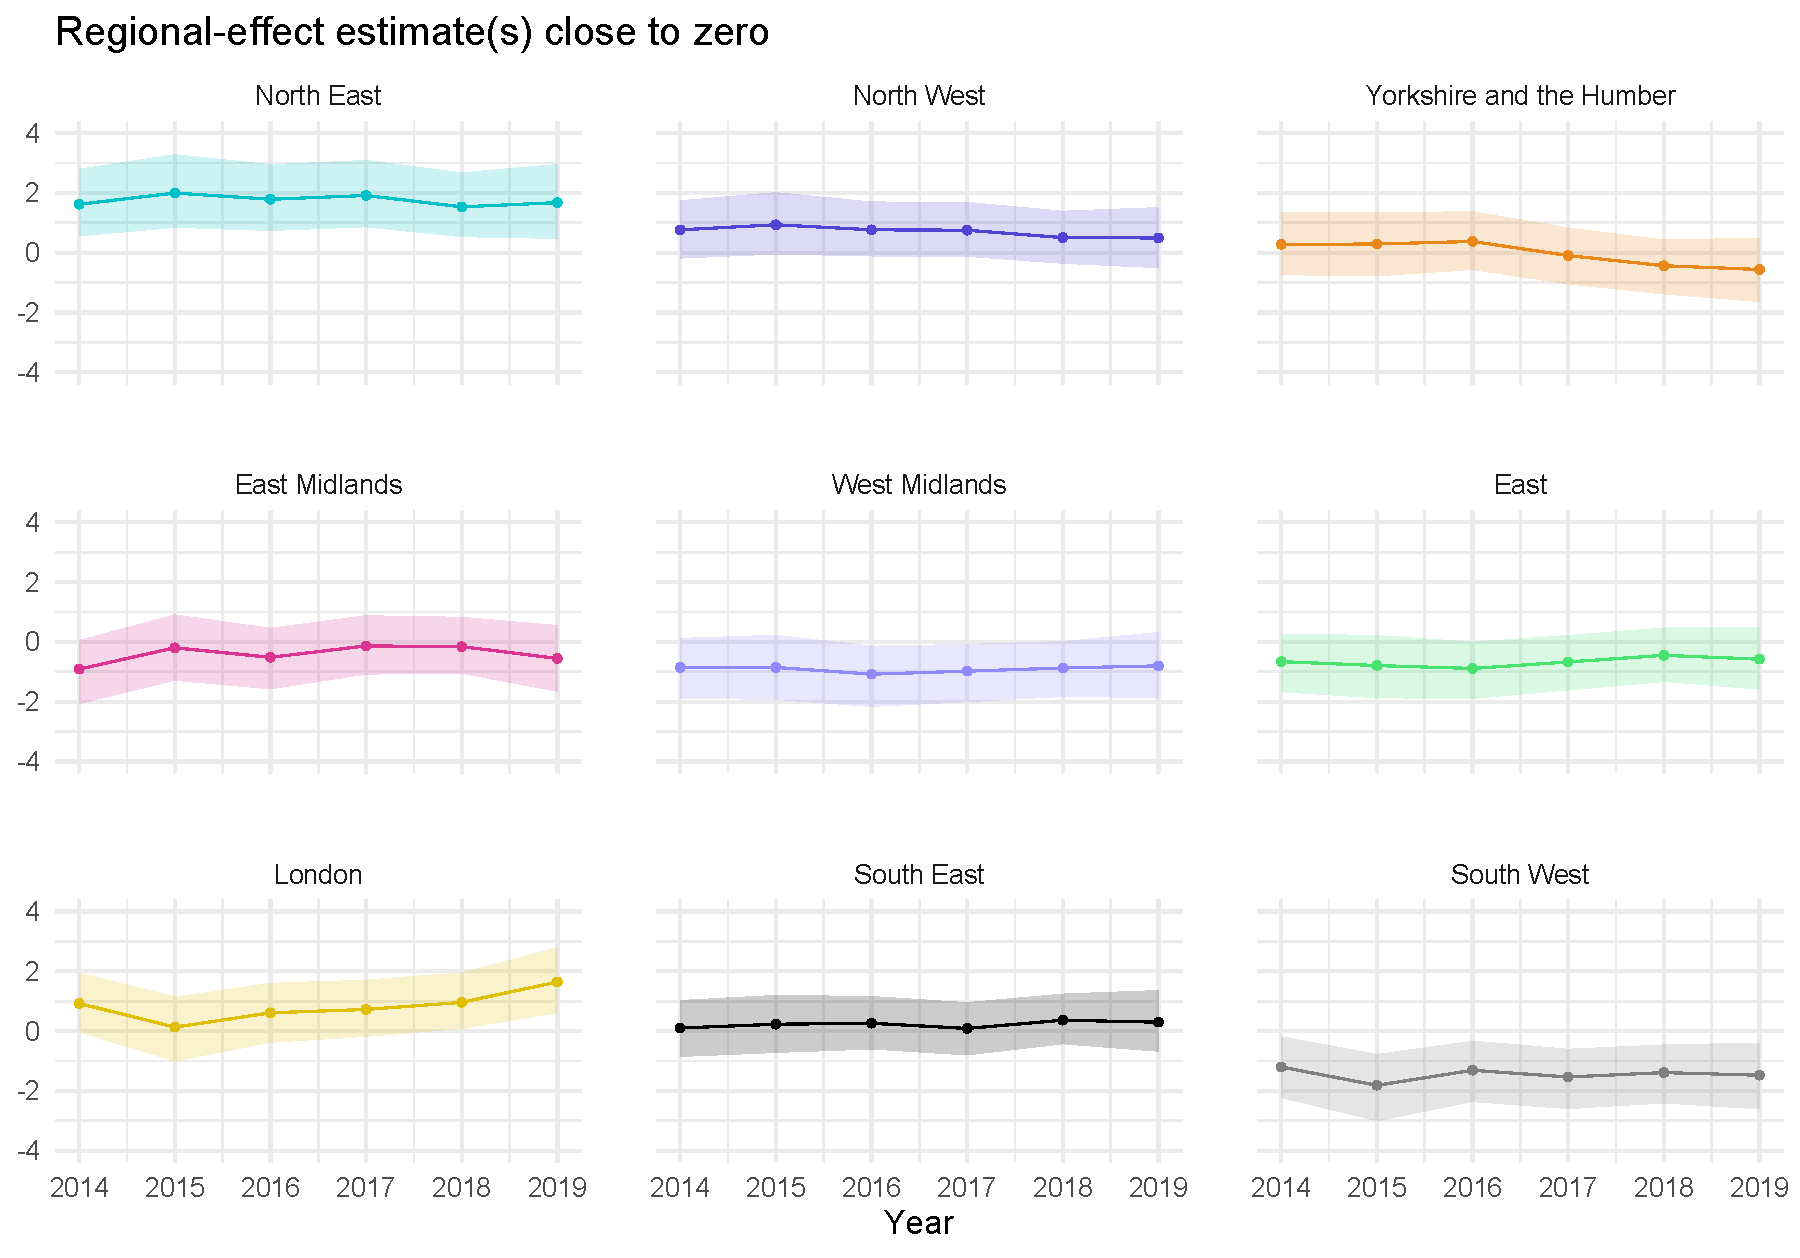
\includegraphics
            [width = \textwidth]
            {fig3_2-1}
        \label{fig:fig3_2-1}
    \end{figure}
\end{frame}